\documentclass[a4paper,12pt]{article}

% for manual date positioning
\usepackage{datetime}
\newdateformat{monthyeardate}{\monthname[\THEMONTH], \THEYEAR}

\usepackage{setspace}   % to change line spacing within a paragraph
%\usepackage{indentfirst}	% to indent first paragraph
\usepackage{graphbox}   % to give includegraph the align option
\usepackage[lmargin=2.00cm,tmargin=3.00cm,rmargin=3.00cm,bmargin=2.00cm,]{geometry}	% for margins
\usepackage[british,english]{babel}	% language
\usepackage{color}	% to specify colours

% for tikz macros
\usepackage{tikz}

% for trademark symbol
\usepackage{textcomp}

\definecolor{sepia}{RGB}{103, 24, 0}

% add float barriers to keep figures from being moved
% http://anorien.csc.warwick.ac.uk/mirrors/CTAN/macros/latex/contrib/placeins/placeins-doc.pdf
\usepackage{placeins}		

% for hyperlinks; colorlinks=true means change the text
% colour rather than adding a colourful border
\usepackage{hyperref} 	
\hypersetup{
  colorlinks=true,
  linkcolor=sepia,
  urlcolor=blue,
}

% paragraph spacing
\setlength{\parskip}{\baselineskip}%

% for lists and margins
\usepackage{enumitem}

% for the author year referencing style, using biber as backend, in citations keep the 
% number of authors to one, then append 'et al.', in bibliography show all authors...
\usepackage[citestyle=ieee,style=authoryear,backend=biber,maxcitenames=1,maxbibnames=20,urldate=short]{biblatex}
\DeclareNameAlias{author}{last-first} % ... with all authors in the `surname, name' format
\addbibresource{bibliography.bib}
\renewcommand*{\nameyeardelim}{\addcomma\space}
\DeclareFieldFormat{urldate}{%
  (visited on: \thefield{urlday}\addspace%
  \mkbibmonth{\thefield{urlmonth}}\addspace%
  \thefield{urlyear}\isdot)}


%%%%%%%%%%%%%%%%%%%%%%%%%%%%%%%%%%%%%%%%%%%%%%%%%%%%%%%%%%%%%%%%%%%%%%

\begin{document}

\begin{titlepage}
  \center
  
  \vspace*{3cm}

  {
    \begin{spacing}{1.2}
      \LARGE The Design and Build of a Simple Personal Finance System, Focused
      on Budgeting and Expenditure Analysis
    \end{spacing}
  }

  \vfill
  
  Word Count: \emph{10,502}, excluding appendices.
  
  \vfill

  Claudius de Moura Brasil\\
  BSc Computing Project Report\\
  Birkbeck College, University of London

  May 2018

  This report is the result of my own work except where explicitly stated in
  the text. The report may be freely copied and distributed provided the source
  is explicitly acknowledged.
  
  \vfill

\end{titlepage}


\newpage
\pagenumbering{roman}
\section{Abstract} \label{sec:Abstract}
Personal finance systems exist in abundance nowadays, from open source to
proprietary ones. They all tend to revolve around a basic common theme:
providing accurate information about an individual's income and expenditure.
Beyond this, they tend to vary in which features are implemented. The system
designed and built for this project focuses on the use of the bookkeeping
principle of double entry and the concept of pattern matching to find effective
ways to cagetorise a user's expenditure, and provide them with relevant
financial information to assist in decision making.


\newpage
\tableofcontents

\newpage
\pagenumbering{arabic}
\section{Introduction} \label{sec:Introduction}

A system could be summarised roughly as a solution to one or more problems. One
of the first steps in order to build this kind of solution is to try to
understand the problem -- that is, try to map the requirements of the software.
Vaasen et al. (2009 \cite[cited][p.~8]{Boczko:2012:IAI:2331376}) suggests that
an accounting information system's main purpose is to provide information to
internal and external stakeholders. Although this refers to accounting systems
for businesses, it could be argued that this same definition can be employed to
define personal finance systems -- except that, in this case, the main
stakeholder would be the individual using the system (that is, the user). In
fact, one of the most widely known accounting systems available in the market,
Quicken\texttrademark, was conceived around the idea that there should be more
efficient and less tedious ways to organise one's personal financial
information than doing it manually (\cite{quicken2017about}). This project has
been developed based on similar ideas.

It seems fair to infer that nowadays most of a user's financial transactions
happen in ways that can be listed electronically (usually via their bank or
credit card statements) -- a study by Payments UK
(\citeyear{paymentsUK2017summary}), for example, indicates that there has been
a rise in debit card payments over the past few years, and that the volumes of
this type of transaction is likely to be higher than that of cash payments by
the year 2021. Therefore, an assumption has been made that the users will
require means of uploading a list of their financial transactions into the
system in an electronic format.

The system created for this project intends to do just this. Its main feature,
however, will be to allow the user to categorise expenditure based on patterns
in the entries' descriptions. Aside from this, there will also be a feature to
allow the user to view summaries of the income and expenditure over a period of
time, and another one to generate budget forecasts for future periods based on
the financial information already entered.

This report documents the work of the project. Each chapter delineates a
specific aspect of the development life cycle, which is in line with the
development process described in the following paragraphs. Chapter
\ref{sec:Requirements} outlines the identified requirements which were used as
motivation for the system to be developed; the contents of Chapter
\ref{sec:AnalysisAndDesign} shows further analysis and concomitant design of
the system and the solutions it brings; Chapter \ref{sec:Implementation}
outlines select aspects of the implementation stage which serve to emphasise
the techniques used to implement the designed logic, or highlights areas where
it was felt it was necessary to implement something slightly different that
what was designed.

The system developed for this project has been modelled after the principle of
\emph{double entry bookkeeping}, from the accounting domain, which states that
``money is never created or destroyed -- it merely moves from one account to
another'' (\cite[][Section 6.2]{fowler1997analysis}). More specifically, double
entry is the principle which ensures that every transaction always affects two
accounts, one being credited (Out) and one debited (In). An account, for the
scope of this project, refers either to a category created by the user, or to
the user's \emph{cash book} -- the contents of their bank account plus any
manual entry which they make. In bookkeeping, each account can be classified as
\emph{asset, liability, income} or \emph{expenditure}. Whether the account
increases or decreases will depend on which of these categories it falls under:
\emph{debits} will increase \emph{assets} and \emph{expense} accounts, and
\emph{credits} will increase \emph{liability, capital} or \emph{income}
accounts (\cite[][pp.~18-19]{wood2004book}).


Regarding the development method, an approach similar to that adopted by
Bennett et al.  (\citeyear[][p.~77]{bennett2010object}) regarding software
analysis an design has been employed, where no specific named methodology is
espoused, but concepts of object-oriented analysis and design were applied, in
an iterative and incremental fashion, using UML. More details about which
concepts were used and the methodologies which originated them can be found in
the following subsections.


The remaining definitions from \hyperref[appendix1]{Appendix I}, including
those of functional and non-functional requirements, will be employed when
trying to classify the requirements and model the problem domain. The initial
iterations will be focused more on the functional and usability requirements,
paying some attention as well to specific non-functional requirements such as
performance and security.

Throughout the report, the term \emph{domain} will be employed, as defined by
Evans (\citeyear[][p.~2]{evans2004domain}), to define the ``activity or
interest of its user'' -- the ``subject area to which the user applies the
program''. 

\hyperref[appendix3]{Appendix III} explains how to build and run the latest
version.


\newpage
\section{Development Method} \label{sec:DevelopmentMethod}
For this project, an approach similar to that adopted by Bennett et al.
(\citeyear[][p.~77]{bennett2010object}) regarding methodology has been
employed, where no specific named methodology is espoused, but concepts of
object-oriented analysis and design were applied, in an iterative and
incremental fashion, using UML. More details about which concepts were used and
the methodologies which originated them can be found in the following
subsections.

\subsection{The use of Universal Modelling Language (UML) constructs}
\label{sec:Introduction.methodology.uml}

UML is a modelling language created with the intention of providing system
architects, software engineers and developers with a common set of modelling
tools, with a defined syntax, which would help them better analyse and design
software-based systems, and to model business and similar processes
(\cite[][p.~43]{omg2015uml}). It defines several constructs which have been
employed throughout this report in order to model the specifications of the
system, such as:
\begin{description}
  \item[Use Case diagrams]
    As a useful, high level tool to document users' requirements
    (\cite[][p.~138]{bennett2010object}), use case diagrams have been used to
    develop the requirements model of the system.

  \item[Activity diagrams]

  \item[Class diagrams]
    
  \item[Sequence diagrams]
\end{description}


\subsection{Requirements Capture Methods} \label{sec:DevelopmentMethod.RequirementsCapture}
Due to the nature of the system being for personal rather than commercial use
-- that is, by individuals rather than business entities -- the usual fact
finding techniques do not apply specifically well. However, the closest match
identified to the techniques utilised has been with \emph{`Knowledge
Acquisition'}. This relates to the process of capturing knowledge from an
expert (\cite[][p.~150]{bennett2010object}). In this particular case, though
perhaps not qualifying as an expert, the author's qualification and experience
in accounting and bookkeeping was used to capture the main requirements.

\subsection{Analysis and Design patterns} Where appropriate, analysis and
design patterns will be used, either in full or with some modifications.

Fowler (\citeyear[][Section~1.3]{fowler1997analysis}) defines a pattern as ``an
idea that has been useful in one context and will probably be useful in
others''. This project will therefore attempt to utilise patterns where
appropriate in order to prove this concept, and as an attempt to make use of
the experience already acquired in the domain (or domains) in question.

The concept of \emph{domain} here is being used, as defined by Evans
(\citeyear[][p.~2]{evans2004domain}), as the ``activity or interest of its
user'' -- the ``subject area to which the user applies the program''.

Analysis patterns will be used ``when trying to understand the problem'' domain
(\cite[][Section~1.1]{fowler1997analysis}).


\newpage
\section{Requirements} \label{sec:Requirements}

\subsection{Business Case} \label{sec:Requirements.BusinessCase}
Any personal accounting system should be able to provide accurate and relevant
summaries of an individual's financial status. In order to do this, the user
needs to be able to supply the system with the necessary data, so that it can
be analysed and properly converted into knowledge.

The scope of the personal finance system developed for this project must
include a feature to allow a user to upload their bank and credit card
statements into it. Each transaction should be classified based on categories
which the user will create. The user should then be able to visualise a summary
of their income and expenditure by category and period, which should allow them
to have a concise and clear visibility of how much they have earned and spent
over any period of time. The category must be handled with care -- there should
not be a case where a user deletes a category and then all the entries in a
period are lost with it, but if a user wants to change the name of a category
they should be free to do so.

Since there may be other sources of income which the user may want to
categorise (such as breakdowns of cash transactions from pocket money), a
feature to allow for manual entries should also be made available. The user can
declare a lump sum, and then break it down among categories. The option should
allow them to choose whether the transaction is a credit or a debit from a
specific category, and then provide the corresponding debit or credit to a
category of their choice. For example, if the user withdraws \pounds50, and
spends half of it on weekly shopping and the other half on a cinema ticket,
they should be able to `credit' (withdraw) \pounds50 from the \emph{Bank}
category, and then `debit' \pounds25 to both \emph{Weekly Shopping} and
\emph{Entertainment} categories.

Once the system has enough data, it should be able to calculate a simple budget
and display it for the user. The budget can be a simple average of income and
expenditure over a long enough period of time, projected over the future
month/year -- it would only be used as a guideline for the user, anyway.

\subsection{Functional Requirements} \label{sec:Requirements.FunctionalRequirements}

Based on the description above, a few functional requirements were identified.
They are represented in the diagram on section
\ref{sec:Requirements.FunctionalRequirements.UseCaseDiagram} and the list,
wireframes and activity diagrams on section
\ref{sec:Requirements.FunctionalRequirements.UseCaseList}.

\subsubsection{Use Case Diagram} \label{sec:Requirements.FunctionalRequirements.UseCaseDiagram}
Use case diagrams are UML constructs which were developed by Jacobson et al.
(1992, cited \cite[][p.~154]{bennett2010object}). The use case diagram on
Figure \ref{fig:UseCaseDiagram} is used to illustrate the functional
requirements identified for this project:
\begin{figure}[ht!]
  \begin{center}
    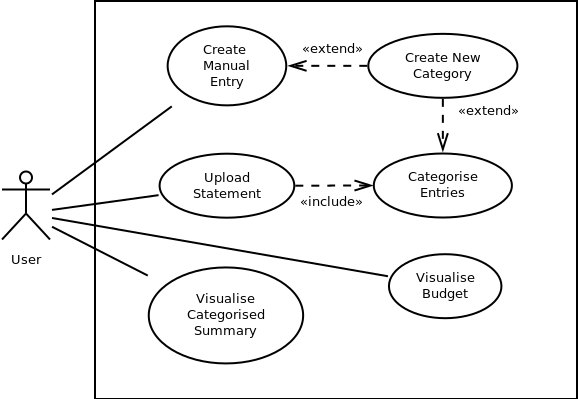
\includegraphics[width=14cm]{./contents/img/Use_Case_Diagram.png}
  \end{center}
  \caption{Use Case Diagram}
  \label{fig:UseCaseDiagram}
\end{figure}
\FloatBarrier



\subsubsection{Use Case List} \label{sec:Requirements.FunctionalRequirements.UseCaseList}
Table \ref{tab:UseCaseDescriptions} lists the descriptions for the use cases
listed above:
\begin{table}[ht!]
  \centering
  \begin{tabular}{|p{4cm}|p{12cm}|}
    \hline
    \textbf{Use Case}&\textbf{Description}\\
    \hline
    Upload Statement&The user must be able to upload a list of their
                     financial transactions, most likely their bank
                     or credit card statements, in a valid format, and all
                     entries should be categorised based on specific patterns\\
                    &\emph{Includes}: Categorise Entries\\
    \hline
    Create Manual Entry&The user should be able to create a manual transaction for
                        income or expenditure, include a date, amount and
                        description, and classify it among existing categories
                        or create new ones in the
                        process\\
                        &\emph{Extends}: Create Category\\
    \hline
    Visualise Categorised Summary&The user must be able to visualise
                                  a summary of their income and expenditure
                                  over a period of time\\
    \hline
    Calculate Budget&The user must be able to visualise a budget for future
                     periods based on their income and expenditure data 
                     already entered\\
    \hline
    Categorise Items&Analyse the current entry and assign it to a category\\
                    &\emph{Extends}: Create Category\\
    \hline
    Create Category&Creates a new category with the name suggested by the
                        user\\

    \hline
  \end{tabular}
  \caption{Use Case Descriptions} \label{tab:UseCaseDescriptions}
\end{table}
\FloatBarrier

The \emph{Estimate Tax} feature  was not included in these requirements, as the
time constraints would not allowed for it to be implemented, but its
specifications can be seen in \hyperref[appendix4]{Appendix IV}.

\subsubsection{Designing the User Experience with Wireframes}
The wireframe below (Figure \ref{fig:Wireframe.CreateManualEntry}) was created
to better illustrate the \emph{Manual Entry} requirement from the point of view
of the user. It shows an example of an entry for a laptop and a licence for a
proprietary operating system, which can then be broken down among different
categories. The user has the option to use the percentage or the amount boxes
in order to provide a breakdown, and they can also add new lines if more than
one is required -- the example shows two lines, but the default would be one.
Under the category search box, if the user types a category name that does not
exist they will be asked if they want to create a new one:
\begin{figure}[ht!]
  \begin{center}
    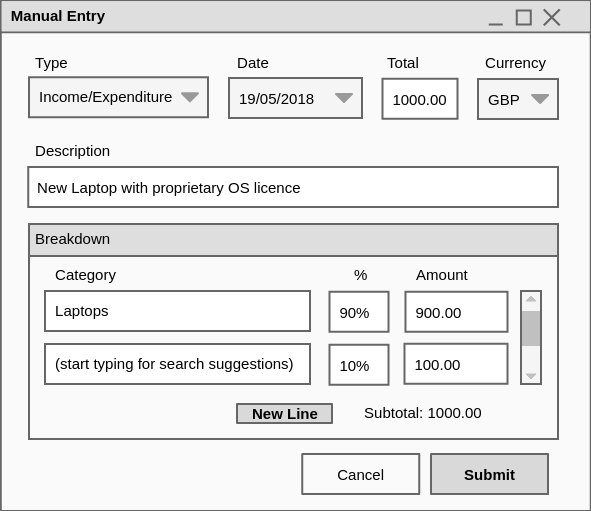
\includegraphics[width=14cm]{./contents/img/Wireframe_-_Manual_Entry.png}
  \end{center}
  \caption{User interface wireframe for \emph{Create Manual Entry} use case}
  \label{fig:Wireframe.CreateManualEntry}
\end{figure}
\FloatBarrier

And in order to better understand the relationship between \emph{Upload
Statement} and \emph{Categorise Entries}, the activity diagram below (Figure
\ref{fig:AD.CategoriseEntries}) was developed:
\begin{figure}[ht!]
  \begin{center}
    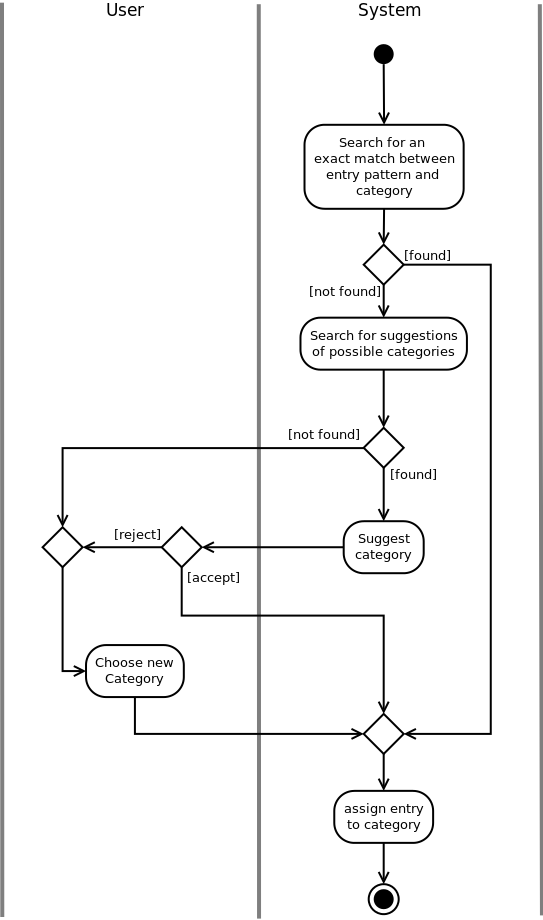
\includegraphics[width=11cm]{./contents/img/Activity_Diagram_-_Categorise_Entries.png}
  \end{center}
  \caption{}
  \label{fig:AD.CategoriseEntries}
\end{figure}
\FloatBarrier

At the first few iterations, in order to provide a minimum viable product, the
process of categorisation will be a blocking one consisting of multiple calls
being made to the process above -- for each call, the process will block awaiting
user input when a category is not found. However, there are plans for future
iterations where this process could be optimised by concurrency, and if there
is enough time a more appropriate interface will be built for such a case.

The initial interface for uploading a statement should be a simple one, such as
the one below
(\ref{fig:Wireframe.UploadStatement}), and at least initially the interface for
manual entry will be used whenever user input is required:
\begin{figure}[ht!]
  \begin{center}
    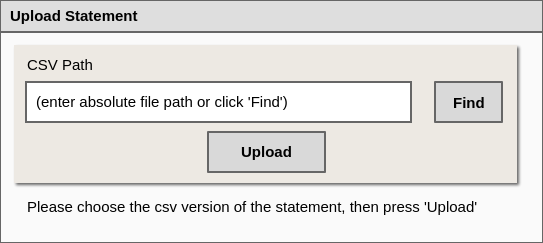
\includegraphics[width=12cm]{./contents/img/Wireframe_-_Upload_Statement.png}
  \end{center}
  \caption{}
  \label{fig:Wireframe.UploadStatement}
\end{figure}
\FloatBarrier

Below (Figure \ref{fig:Wireframe.VisualiseCategorisedSummary}) is also a
wireframe illustrating the GUI for \emph{Visualise Categorised Summary}. The
user should have an option to select the dates and, if they only want to see
one category, the category itself:
\begin{figure}[ht!]
  \begin{center}
    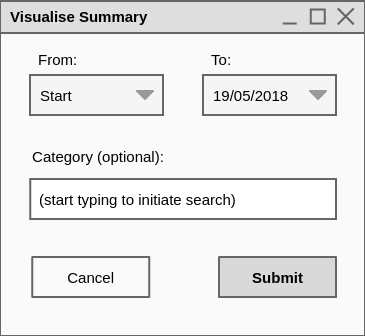
\includegraphics[width=8cm]{./contents/img/Wireframe_-_Visualise_Summary.png}
  \end{center}
  \caption{}
  \label{fig:Wireframe.VisualiseCategorisedSummary}
\end{figure}
\FloatBarrier

The dates field should allow them both to type a date or choose it from a drop
down calendar. If no values are entered, the system will return a summary of
all categories on the system.




\subsection{Non-Functional Requirements} \label{sec:Requirements.NonFunctionalRequirements}
At this iteration, no significant non-functional requirements were identified,
so they were not included in this report.


\newpage
\printbibliography[heading=bibintoc]

\end{document}
